%------------------------------------------------------------------------
% Template provided by MIT
%------------------------------------------------------------------------
\documentclass[12pt,twoside]{mitthesis}
%------------------------------------------------------------------------
\usepackage{ragged2e}
\usepackage{biblatex}
\usepackage[nottoc,notlot,notlof]{tocbibind}
\usepackage{amssymb}
\usepackage{indentfirst}
\usepackage{graphicx}
\usepackage{caption}
%------------------------------------------------------------------------
\begin{document}
%------------------------------------------------------------------------
% Renew commands - Translation
%------------------------------------------------------------------------
\renewcommand{\labelitemi}{\tiny$\blacksquare$}
\renewcommand{\bibname}{Bibliograf\'ia} 
\renewcommand{\abstractname}{Abstract}
\renewcommand{\contentsname}{Tabla de Contenido}
\renewcommand{\listtablename}{Lista de Tablas} 
\renewcommand{\listfigurename}{Lista de Figuras}
\captionsetup[table]{name = Tabla,font=small,skip=0pt} 
%------------------------------------------------------------------------
% Add captions
%------------------------------------------------------------------------
% \captionsetup[table]{name = Tabla}
%------------------------------------------------------------------------
% Document Structure
%------------------------------------------------------------------------
	\department{Escuela de Ingenier\'ia en Computaci\'on}
\degree{Programa de Maestr\'ia en Computaci\'on.}
\title{{\large\bf{Cubic Spline Interpolation como medida de distancia utilizada en el descubrimiento de reglas significativas en series temporales complejas y en presencia de ruido}}}
\author{David El\'ias Alfaro Barboza}
\supervisor{Luis Alex\'ander Calvo Valverde}{Supervisor}
\auditor{Luis Alex\'ander Calvo Valverde}
\degreemonth{Julio}
\degreeyear{2016}
\thesisdate{Julio 2016}
\maketitle
\begin{abstractpage}
% $Log: abstract.tex,v $
"El abstract se escrib\'ira aqu\'i"
\end{abstractpage}	
%\section*{Acknowledgments}

%------------------------------------------------------------------------
\tableofcontents
%\newpage
%\listoffigures
%\newpage
%\listoftables
%------------------------------------------------------------------------


\listoftables
\let\cleardoublepage\clearpage
\listoffigures
\let\cleardoublepage\clearpage
\section{\textbf{Introducci\'on}}
La habilidad de hacer predicciones acerca de acontecimientos o eventos de la vida real ha sido siempre un tema de gran inter\'es para la ciencia.\par 
En la \'ultima d\'ecada, la comunidad de miner\'ia de datos se ha interesado vehementemente en el hallazgo de patrones o reglas que puedan ser \'utiles en la predicci\'on de eventos de corto y de largo plazo \cite{main}.\par
La mayor\'ia de trabajos de investigaci\'on recientes, orientados en la predicci\'on de eventos de corto plazo mediante series temporales, se han enfocado principalmente en el an\'alisis de los \textit{\textbf{valores actuales}} del flujo de datos \cite{rulediscovery}\cite{subsequencematching}. Sin embargo, en una basta cantidad de casos, el an\'alisis de los valores actuales es irrelevante; en su lugar, la \textit{\textbf{forma}} actual del patr\'on o la regla motivo y la detecci\'on oportuna en el flujo de datos, pueden ayudar a anticipar la ocurrencia de eventos futuros con mayor precisi\'on \cite{main}.\par
Este trabajo de investigaci\'on tiene como objetivo principal, la implementaci\'on de la medida de distancia llamada \textit{Cubic Spline Interpolation} en los algoritmos \textit{\textbf{\enquote{Rule Bit Saves}}} y \textit{\textbf{\enquote{Find Antecedent Candidates}}}, utilizados respectivamente en el hallazgo y la detecci\'on de reglas significativas, para llevar a cabo predicciones de corto plazo, sobre series temporales complejas y en presencia de ruido.\par
Las predicciones de corto plazo sobre series temporales han tenido un auge importante, su aplicaci\'on y alcance se ha diversificado considerablemente. Las predicciones de corto plazo sobre texto durante las pulsaciones del teclado, predicciones sobre consultas de base de datos \cite{type}, predicciones sobre intervenciones m\'edicas \cite{medical}, son solo algunos ejemplos de predicciones sobre objectos discretos.\par
Recientemente, ha surgido una reto a\'un mayor; se requiere un mayor poder predictivo, lo que implica necesariamente la implementaci\'on de algoritmos de predicci\'on mucho m\'as precisos, m\'as veloces y que puedan hallar patrones sobre conjuntos de datos mucho m\'as grandes y complejos \cite{robotics}. Por ejemplo, el radar Doppler utilizado en las \'ultimas dos d\'ecadas para la detecci\'on de tornados, ha incrementado el tiempo promedio de alerta de 5.3 a 9.5 minutos, salvando un incontable n\'umero de vidas humanas a\~no con a\~no. Sin embargo, a\'un se reportan alrededor de un 26\% de tornados que no pueden predecirse mediante el uso de la tecnolog\'ia existente \cite{weatherforcasting}. McGovern et al. argumentan en \cite{weatherprediction}, que las nuevas mejoras no vendr\'an necesariamente de sensores m\'as sofisticados, sino, de algoritmos de predicci\'on a\'un no inventados o algoritmos existentes a\'un no depurados, capaces de examinar series temporales complejas, para hallar reglas predictivas mucho m\'as precisas y fiables.\par
La presente propuesta de investigaci\'on se encuentra distribu\'ida de la siguiente manera: inicialmente, en la secci\'on cuatro, se desarroll\'a el marco te\'orico como un grupo de ideas y conceptos fundamentales, que tienen como objetivo principal, guiar e involucrar al lector en el contexto de esta propuesta de investigaci\'on. En la secci\'on cinco, se exponen los detalles m\'as importantes de la propuesta de investigaci\'on, tales como el planteamiento del problema, la hip\'otesis, las m\'etricas utilizadas y del por qu\'e la importancia de llevar a cabo esta investigaci\'on. El objetivo general y los objetivos espec\'ificos de esta propuesta, se ofrecen en las secciones seis y siete respectivamente. El alcance y las limitaciones, ser\'an puntualmente detalladas en la secci\'on ocho, mientras que los entregables ser\'an enlistados en la secci\'on nueve. Por otra parte, en la secci\'on diez, se describir\'a el dise\~no experimental y el ambiente de desarrollo que le dar\'an forma a la metodolog\'ia utilizada. Finalmente, en la secci\'on once, se presenta el cronograma de actividades establecido, para la llevar a cabo la realizaci\'on de este proyecto de investigaci\'on.
\section{\textbf{Propuesta de Proyecto}}
\subsection{Planteamiento del Problema}
El c\'alculo de la similitud en series temporales ha sido un tema muy estudiado en la \'ultima d\'ecada \cite{rulediscovery}. La precisi\'on, la velocidad de c\'omputo y la tolerancia al ruido, son factores claves (particularmente en conjuntos de datos grandes y complejos) a la hora de elegir una medida de distancia robusta para comparar dos series de tiempo de largo n \cite{multidimensional}.\par
En la literatura, la medida de distancia m\'as utilizada para comparar series temporarles es sin duda la distancia \textit{Euclidiana} (o alguna de sus variaciones). Dicha medida es muy utilizada en el descubrimiento y la comparaci\'on de reglas motif o patrones en series temporales \cite{motifs}\cite{patterns}.\par
Existen pruebas emp\'iricas fiables, que demuestran que la distancia Euclidiana es muy competitiva e incluso superior a medidas mucho m\'as complejas en una amplia variedad de dominios, particularmente cuando el conjunto de datos se vuelve cada vez m\'as grande \cite{distancecomparison}\cite{timewarpingindexing}.\par
Sin embargo, algunos aportes m\'as recientes al estado del arte indican que  \textit{Dynamic Time Warping}, en una o varias dimensiones, puede incluso comportarse de forma m\'as robusta y estable que la distancia \textit{Euclidiana} \cite{keogh}. Este argumento se soporta principalmente en la sensibilidad conocida que presenta la distancia \textit{Euclidiana} ante la presencia de ruido, pero fundamentalmente y por su naturaleza lineal \cite{euclidean}, intolerante ante peque\~nas distorciones observadas al comparar dos series temporales desfasadas con respecto al eje tiempo \cite{DTWcubicsplineinterpolation}.\par
Por \'ultimo, la presencia de ruido y de valores faltantes en los datos de una serie de tiempo, son problemas dif\'iciles de tratar; lo que s\'i es seguro, es que son retos inevitables, pr\'acticamente inherentes, que al igual que las limitaciones de las medidas de distancia, deben abordarse previo al an\'alisis y que, finalmente definen el planteamiento del problema \cite{noise}.\par
El problema anteriormente planteado, se atacar\'a mediante la siguiente propuesta de investigaci\'on.
\subsection{Propuesta del Proyecto}
Apoyados en la premisa anterior, el proyecto pretende estudiar el nivel de acierto obtenido como resultado del descubrimiento de \textit{\enquote{reglas significativas}} en series de tiempo, utilizando \textit{Cubic Spline Interpolation} como una medida alternativia de distancia aparentemente superior a la distancia \textit{Euclidiana}, principalmente ante la presen\-cia de distorciones en el conjunto de datos y otras limitaciones ya planteadas.\par
El proyecto se enfoca en remplazar la distancia Euclidiana y probar que la utilizaci\'on de otras medidas de distancia (particularmente el uso de \textit{Cubic Spline Interpolation}) pueden ser mucho m\'as tolerantes al ruido y a\'un as\'i, garantizar al menos el mismo nivel de acierto en el descubrimiento de reglas significativas en series temporales.
\subsection{Trabajos Relacionados}
La presente propuesta de investigaci\'on se basa en trabajo de Mohammad Shokoohi-Yekta et al \cite{main}, quienes proponen una serie de nuevos algoritmos que permiten el des\-cubrimiento veloz de reglas significativas de alta calidad a partir de grandes conjuntos de datos, las cuales, pueden predecir la ocurrencia de eventos futuros.\par
Es importante destacar el hecho de que \textit{\textbf{todos los algoritmos propuestos en \cite{main} utilizan la distancia Euclidiana}} para la identificaci\'on de reglas motif y su selecci\'on posterior como reglas significativas.\par
A diferencia de otras propuestas mencionadas a continuaci\'on, el trabajo propuesto en \cite{main}, se basa el descubrimiento de reglas motif basadas en \textit{la forma} para vaticinar los eventos futuros. En contraposici\'on, los trabajos anteriores intentan lograr predicciones basadas en los \textit{valores actuales} del flujo de datos \cite{others}.\par
En una secuencia de trabajos que culminaron en \cite{elasticrules}, Park y Chu, investigaron un mecanismo para hallar reglas sobre series de tiempo. Sin embargo, el algoritmo \'unicamente es valorado con respecto a la velocidad y datos aleatorios (\textit{random walk data}). No se presentaron pruebas de que el algoritmo pudiera en realidad encontrar las reglas generalizables en series de tiempo.\par
Los trabajos de Wu y colegas en \cite{eventdriven}, tambi\'en utilizan representaciones lineales de segmentos para apoyar el descubrimiento de reglas en series de tiempo. Ellos probaron su algoritmo sobre datos financieros reales, reportando aproximadamente un 68\% de \enquote{correcci\'on de la predicci\'on de la tendencia de datos} sobre la serie temporal. Curiosamente, sin embargo, los autores corrieron su algoritmo en datos proporcionados por otros y obtuvieron exactamente los mismos resultados.\par


\subsection{Hip\'otesis}
Con base en la definici\'on del problema y en la propuesta de proyecto, se define la siguiente hip\'otesis:\par
\textbf{\textit{El uso de la medida de distancia \textit{Cubic Spline Interpolation}, mejora el nivel de exactitud en los algoritmos \textit{\textbf{\enquote{Rule Bit Saves}}} y \textit{\textbf{\enquote{Find Antecedent Candidates}}} propuestos por Mohammad Shokoohi-Yekta y colaboradores, en el hallazgo de reglas significativas en series de tiempo complejas y en presencia de ruido.}} 
\subsection{M\'etricas}
El an\'alisis comparativo de los niveles de exactitud obtenidos a partir de la ejecuci\'on de los algoritmos seg\'un la distancia utilizada, requerir\'a de las siguientes m\'etricas:
\begin{itemize}
\item \textbf{Exactitud (Q):}
\begin{equation}
 \frac{Total\_Aciertos} {Total\_Predicciones}
\end{equation}
\end{itemize}
En el caso m\'as general, se utilizar\'a inicialmente la distancia Euclidiana entre la parte consecuente predicha y las \textit{\textbf{F}} ubicaciones halladas desde donde la regla fue disparada, un valor denotado como \textit{\textbf{\enquote{Ferror}}}, tambi\'en conocido como la \textit{media cuadr\'atica}.\par
Sobre el mismo conjunto de prueba, y mediante el uso del mismo segmento consecuente de la regla, se disparar\'a aleatoriamente \textit{\textbf{F}} veces y se medir\'a la distancia \textit{Euclidiana} (Cubic Spline Interpolation y otras ya mencionadas en el marco te\'orico), entre el segmento consecuente predicho y la ubicaciones aleatorias F.\par
Ese valor ser\'a denotado como \textit{\textbf{Rerror}} (el cual, se promediar\'a entre aproximadamente 1000 ejecuciones aleatorias).\par
En resumen, la medida de calidad reportada puede definirse como: 
\begin{equation} 
Q = \frac{Ferror}{Rerror} 
\end{equation}
Los valores cercanos a uno, sugieren que las reglas a prueba, no se consideran mejores que las encontradas en la estimaci\'on aleatoria. Los valores significativamente menores a uno, indican que la regla en efecto encuentra una estructura verdadera en los datos. En la mayor\'ia de los experimientos se utilizar\'a un retraso m\'aximo (\textit{\textbf{maxlag}}) \cite{main} igual a cero.
\subsection{Justificaci\'on del Proyecto}
La realizaci\'on de este proyecto es importante, porque a trav\'es de sus resultados se podr\'ian llegar a obtener los siguientes beneficios:
\begin{itemize}
\item {\textbf{\textbf{Un aporte al estado del arte}}. El estudio del estado del arte realizado indica que \enquote{Cubic Spline Interpolation}, como medida de distancia, no ha sido utilizado a\'un en algoritmos para el descubrimiento de reglas significativas sobre series temporales. La idea es, por ende, prometedora e innovadora y podr\'ia tener un impacto significativo sobre el rendimiento de algoritmos existentes que actualmente utilizan otras medidas de distancia m\'as utilizadas como por ejemplo, la distancia \textit{Euclideana}.}
\item {\textbf{Ataca un problema de investigaci\'on real}. Muchas de las aplicaciones producto del an\'alisis de series temporales, son posibles a partir del descubrimiento de reglas \textit{motif} y su uso posterior sobre el conjunto de datos \cite{main}. El descubrimiento de dichos patrones en series temporales, se puede resumir a un problema de \textit{similitud}. El c\'omputo de la similitud (o disimilitud) se obtiene a partir de la medida de distancia entre los puntos de datos de las series temporales \cite{main}. Mientras m\'as eficiente y robusta sea la medida de distancia, mejor ser\'a el c\'alculo de la similitud y por ende, mejores reglas \textit{motif} se obtendr\'an. Como consecuencia de lo anterior, la precisi\'on, la velocidad del c\'omputo y la tolerancia al ruido ser\'an superior y por consiguiente, la calidad predictiva de la regla sobre el conjunto de datos ser\'a mucho m\'as fiable \cite{measurements}.}
\item {\textbf{Las potenciales aplicaciones y su impacto en la sociedad}. Como se desarroll\'o en el marco te\'orico, las aplicaciones de la miner\'ia sobre series temporales son amplias y diversas  \cite{main}. Las predicciones de corto plazo mediante el uso de reglas significativas en campos triviales como el an\'alisis del mercado de accio\-nes, el estudio de las condiciones meteorol\'ogicas (por ejemplo, el incremento del tiempo promedio de alerta de tornados \cite{weatherforcasting}) son cada d\'ia m\'as utilizadas. En rob\'otica, por ejemplo, se han realizado avances significativos en la exploraci\'on de la anticipaci\'on (predicciones de corto plazo) de las fuerzas futuras percibidas por un robot con base en las intenciones motoras de otro agente y as\'i adaptar su movimiento, ejecutando un nuevo plan de acci\'on \cite{robotics}.}
\end{itemize}
\section{\textbf{Objetivo General}}
El objetivo general de esta propuesta de investigaci\'on es: estudiar el nivel de exactitud obtenido al utilizar \textit{Cubic Spline Interpolation} como medida de distancia utilizada en el descubrimiento de reglas significativas en series temporales complejas y en presencia de ruido.
\section{\textbf{Objetivos Espec\'ificos}}
Los objetivos espec\'ificos de este proyecto son los siguientes:
\begin{itemize}
\item [1.] Proponer el uso de \textit{Cubic Spline Interpolation} como medida de distancia utilizada en los algoritmos creados por Mohammad Shokoohi-Yekta y colaboradores (\textit{\textbf{\enquote{Rule Bit Saves}}} y \textit{\textbf{\enquote{Find Antecedent Candidates}}}), para el descubrimiento de reglas significativas en series temporales complejas y en presencia de ruido.
	\item [2.] Realizar un an\'alisis comparativo del nivel de exactitud obtenido al utilizar diferentes medidas de distancia en los algoritmos mencionados.
\item [3.] Explicar los resultados obtenidos en el objetivo espec\'ifico anterior, con el prop\'osito de aprobar o rechazar la hip\'otesis planteada.
\end{itemize}
\section{\textbf{Alcance y Limitaciones}}
El alcance de esta propuesta de investigaci\'on se enfoca espec\'ificamente en estudiar el efecto de utilizar \textit{\enquote{Cubic Spline Interpolation}} como medida de distancia en los algoritmos \textit{\textbf{\enquote{Rule Bit Saves}}} y \textit{\textbf{\enquote{Find Antecedent Candidates}}} propuestos por Mohammad Shokoohi-Yekta y colaboradores, utilizados para el hallazgo de reglas significativas en series de tiempo complejas y en presencia de ruido.\\
El dise\~no experimental incluye tambi\'en la comparaci\'on y el an\'alisis de cinco versiones de ambos algoritmos. Cada versi\'on incorpora la implementaci\'on de cinco medidas de distancia distintas: 1- Euclideana, 2- Swale, 3- Spade, 4- EPR y 5- Cubic Spline Interpolation.\\
Como resultado de esta investigaci\'on, se entregar\'an los siguientes productos:
\begin{itemize}
\item La implementaci\'on de las cinco versiones de ambos algoritmos para cada una de las medidas de distancia.
\item Programas auxiliares para la ejecuci\'on y el control del entregable anterior.
\item An\'alisis estad\'istico para constrastar los resultados de los experimentos.
\item Un art\'iculo cient\'ifico que se entregar\'a al comite editorial de alguna revista o conferencia, con miras a su publicaci\'on.
\end{itemize}
Es necesario delimitar esta investigaci\'on por motivos de tiempo y extensi\'on. Es por ello que a continuaci\'on se detallan las siguientes limitaciones:
\begin{itemize}
\item No se tomar\'an en cuenta otras medidas de distancia.
\item No se utilizar\'a ning\'un otro algoritmo para la identificaci\'on de reglas \textit{motif}.
\item No se utilizar\'a ning\'un otro algoritmo para la detecci\'on de segmentos antecedentes de una potencial regla significativa.
\item Cualquier otro resultado, documento, software o producci\'on que no se encuentren contemplados en los entregables, no ser\'a considerado como parte del alcance de este proyecto.
\end{itemize}
En resumen, debe considerarse el hecho de que el objetivo principal de esta investigaci\'on, se enfoca principalmente en la implemetaci\'on de las medidas de distancia sobre ambos algoritmos, para su posterior an\'alisis comparativo, aplicado a cada unos de los cinco diferentes conjuntos de datos; utilizando \textit{\enquote{Cubic Spline Interpolation}} como el elemento m\'as importante de la hip\'otesis planteada.
\section{\textbf{Entregables}}
Los entregables son los siguientes:
\begin{itemize}
\item \textbf{Modificaci\'on del software utilizado para el hallazgo de reglas significativas:} incorporar las medidas de distancia propuestas para ambos algoritmos.
\item \textbf{Desarrollo e implementaci\'on de un ambiente de pruebas:} este ambiente permitir\'a ejecutar y medir la exactitud de ambos algoritmos, en el hallazgo y la selecci\'on de reglas significativas.
\item \textbf{Documento final con la recopilaci\'on y el an\'alisis del dise\~no de experimentos:} este entregable implica la ejecuci\'on del dise\~no de experimentos y la construcci\'on de un tabla resumen de los resultados obtenidos. 
\item \textbf{Documento final del an\'alisis de varianza no param\'etrico y la caracterizaci\'on de los resultados obtenidos:} corresponde al an\'alisis de varianza no param\'etrico, para aceptar o rechazar la hip\'otesis mediante la caracterizaci\'on de los resultados.
\item \textbf{Documento de tesis:} recopila los entregables anteriores, las conclusiones y el resultado de la revisi\'on de la hip\'otesis. Incluye adem\'as, el desarrollo de un art\'iculo cient\'ifico.
\item \textbf{Preparaci\'on de la defensa:} crear una presentaci\'on (\textit{Beamer}) que resuma los aspectos m\'as destacados de esta investigaci\'on.
\end{itemize}
\section{\textbf{Metodolog\'ia}}
\subsection{Dise\~no de Experimentos}
Para describir el planeamiento pre-experimental para el dise\~no de experimentos de este trabajo, (con la informaci\'on disponible hasta el momento), se usan los \textit{lineamientos} desarrollados en el libro de Douglas C. Montgomery [2]. El esquema del procedimiento recomendado en los lineamientos para el desarrollo de esta etapa incluye lo siguiente:
\begin{itemize}
\item [1.] \textbf{Reconocimiento y definici\'on del problema:} consiste en desarrollar una declaraci\'on clara y sencilla del problema. Una clara definici\'on del problema, normalmente contribuye substancialmente a una mejor comprensi\'on del fen\'omeno que esta siendo estudiado y a la soluci\'on final de dicho problema.
\item [2.] \textbf{Selecci\'on de factores, niveles y rangos:} consiste en enumerar todos los posibles factores que pueden influenciar el experimento. Incluye tanto los factores de dise\~no potencial (los que potencialmente se podr\'ian querer modificar en los experimentos) y los factores perturbadores (los que no se quieren estudiar en el contexto del experimento). Tambi\'en se deben seleccionar los rangos sobre los que var\'ian los distintos factores y los niveles espec\'ificos sobre los que se aplicar\'an las iteraciones del experimento.
\item [3.] \textbf{Selecci\'on de la variable de respuesta:} debe proveer informaci\'on \'util sobre el fen\'omeno que esta siendo estudiado.
\item [4] \textbf{Selecci\'on del dise\~no de experimental:} se refiere a aspectos claves del experimento tales como el tama\~no de la muestra, la selecci\'on del orden adecuado para la ejecuci\'on de los intentos experimentales y la decisi\'on de bloquear o no algunas de las restriciones de aleatoriedad en la pruebas.
\item [5] \textbf{Llevar a cabo el experimiento:} en esta etapa, es de vital importancia monitorear el proceso cuidadosamente para asegurar la correcta ejecuci\'on del experimento con respecto a lo planeado.
\end{itemize}
\subsubsection{Declaraci\'on del Problema}
Estudiar el comportamiento de \textit{Cubic Spline Interpolation} como medida de distancia utilizada en el descubrimiento de reglas significativas en series temporales complejas y en presencia de ruido.\\
\textit{Cubic Spline Interpolation} y otras medidas medidas de distancia ser\'an incorporadas en dos los algoritmos espec\'ificos llamados \textit{\textbf{"Rule Bit Saves"}} y \textit{\textbf{"Find Antecedent Candidates"}} propuestos por Mohammad Shokoohi-Yekta y colaboradores.\\
Por cada medida de distancia utilizada, se crear\'a una nueva versi\'on de ambos algoritmos.\\
La precisi\'on en el hallazgo de reglas significativas ser\'a medido a trav\'es de la ejecuci\'on, la comparaci\'on y el an\'alisis de cada version de version de los algoritmos, mediante la utilizaci\'on de al menos cinco fuentes de datos temporales de complejidad variada y en presencia de diferentes niveles de ruido.
\subsubsection{Factores y Niveles}
En el dise\~no de experimentos, un factor es aquel componente que tiene cierta
influencia en las variables de respuesta [2].\\
El objetivo de un experimento es determinar esta influencia. A su vez, cada factor cuenta con varios niveles posibles con los cuales experimentar.\\
Usando la informaci\'on recolectada en esta etapa de la investigaci\'on, as\'i como la experiencia adquirida por el estudiante y expuesta en los cap\'itulos anteriores, se han seleccionado inicialmente los siguientes dos factores para su estudio:
\begin{itemize}
\item [1.] \textbf{Las m\'etricas o medidas de distancia}\\
Se utilizar\'an dos algoritmos para la ejecuci\'on del dise\~no de experimental: 1- \textit{\textbf{"Rule Bit Saves"}} utilizado en la selecci\'on de potenciales reglas o patrones significativos (\textit{\textit{detecci\'on de reglas \textit{Motif [1]}}}) y 2- \textit{\textbf{"Find Antecedent Candidates"}}, creado para probar la efectividad de las reglas m\'as significativas sobre cada uno de los conjuntos de datos.\\
Ambos algoritmos ser\'an moficados y adaptados a cada medida de distancia y su ejecuci\'on sobre cada conjunto de datos ser\'a realizada en forma controlada e independiente.\\
Las medidas de distancia utilizadas, son las siguientes:
\begin{itemize}
\item \textbf{\textit{Distancia Euclidiana}}
\item \textbf{\textit{Swale}}
\item \textbf{\textit{Spade}}
\item \textbf{\textit{EPR}}
\item \textbf{\textit{Cubic Spline Interpolation}}
\end{itemize}
\item [2.] \textbf{El conjunto de datos, tama\~no y complejidad}\\
Con respecto a la cantidad de ruido encontrado en el conjunto de datos, podemos definir al menos tres diferentes tama\~no: 1- conjunto de datos con poco ruido (nivel pendiente de determinar), 2- conjunto de datos con ruido moderado (nivel pendiente de determinar), 3-conjunto de datos con mucho ruido (nivel pendiente de determinar). \\
En el experimento, se utilizar\'an los siguientes conjuntos de datos:
\begin{itemize}
\item 1. \textbf{Energy disaggregation dataset:} contiene el amperaje del consumo diaro de una casa promedio durante un a\~no.
\item 2. \textbf{Zebra finch vocalizations:} contiene las grabaciones del canto de un pajaro Zebra durante sus primeros 100 d\'as.
\item 3. \textbf{Daily basis activity data set:} este conjunto de datos contiene informaci\'on telem\'etrica de actividades cotidianas de una persona.
\item 4. \textbf{NASA telemetry data:} contiene medidas de voltajes err\'oneas producidas por las v\'alvulas utilizadas en los transbordadores espaciales de la NASA, utilizadas para el estudio y la detecci\'on de anomal\'ias .
\end{itemize}
\end{itemize}
\begin{center}
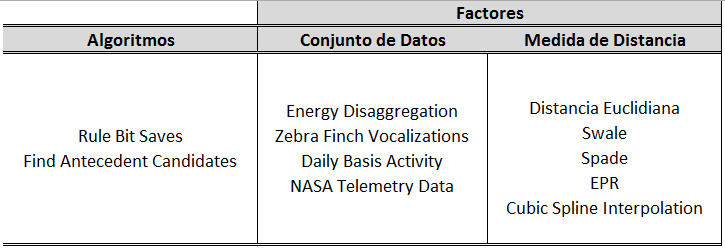
\includegraphics[scale=0.7]{factors.png}\\
\vspace*{10pt}
\footnotesize{\textbf{Imagen 1.} Tabla de factores por analizar en esta investigaci\'on.}
\end{center}
\subsubsection{Variables de Respuesta}
Dado que la hip\'otesis afirma maximizar el nivel de exactitud en la selecci\'on y el hallazgo de reglas significativas, se han seleccionado las siguientes variables de respuesta:
\begin{itemize}
\item [1.] \textbf{\textit{Exactitud:}} total de aciertos en la identificaci\'on de reglas \textit{motif} (potenciales reglas significativas), sobre cada conjunto de prueba, mediante la ejecuci\'on de las diferentes versiones del algoritmo \textbf{"Rule Bit Saves"}.
\item [2.] \textit{\textbf{Precisi\'on:}} mide la calidad de la medida de distancia para cada version del algoritmo \textit{\textbf{"Find Antecedent Candidates"}}, en la detecci\'on del segmento antencedente de la regla sobre el flujo de datos, para cada conjunto de datos de prueba.
\end{itemize}
\subsubsection{Recolecci\'on de Datos}
Las variables de respuesta ser\'an recolectadas de forma autom\'atica una vez concluida la ejecuci\'on de cada una de las versiones de ambos algoritmos.\\
La automatizaci\'on de la recolecci\'on de las variables de respuesta ser\'a posible mediante la implementaci\'on del ambiente de pruebas.
\subsubsection{An\'alisis de Varianza}
Una vez conclu\'ida la ejecuci\'on del experimento, se deben analizar los resultados para compar ambos algoritmos en sus diferentes versiones. Para esta comparaci\'on, se debe analizar si existe una diferencia significativa en los promedios obtenidos de una determinada variable de respuesta para cada uno de los distintos grupos. Un an\'alisis de varianza permite saber si la diferencia en la media de varias poblaciones es significativa debido a la influencia de alguno de los factores.\\

\subsection{Ambiente de Desarrollo}
Para el desarrollo de la tesis, se implementar\'a una plataforma que cumpla con dos caracter\'isticas principales:
\begin{itemize}
\item [1.] Que la plataforma se pueda ejecutar sobre los sistemas operativos Windows y Linux: esto implica que el c\'odigo fuente debe ser escrito en un lenguaje de programaci\'on capaz de correr en los dos sistemas operativos con un n\'umero m\'inimo de cambios y que las bibliotecas utilizadas est\'en disponibles para los dos sistemas operativos.
\item [2.] Que las herramientas y bibliotecas a utilizar sean gratuitas al menos para uso acad\'emico.
\end{itemize}
Basado en estas dos caracter\'isticas, se ha elegido una lista de posibles soluciones de software a utilizar. Como se indica, esta lista es preliminar, por lo que se preveen posibles cambios durante el desarrollo de la tesis.
\begin{itemize}
\item \textbf{Sistema Operativo:} Windows 8.1.
\item \textbf{Lenguaje de programaci\'on:} Matrix Laboratory (MATLAB).
\end{itemize}

\section{\textbf{Plan de Trabajo}}
El plan de trabajo para esta investigaci\'on es la secuencia de pasos por ejecutar
para generar los entregables mencionados en la secci\'on 6 de este documento.\\
El curso de tesis 2 del TEC est\'a dise\~nado para ser ejecutado en un periodo de \textit{16 semanas}, por lo que es necesario planificar estos pasos de forma tal que sea posible realizarlos en el tiempo esperado con una alta probabilidad de \'exito.
\section{Lista de Tablas}
\begin{table}[h]
\caption{Listado de entregables, objetivos relacionados y duraci\'on}
\label{arm:tabla}
\begin{center}
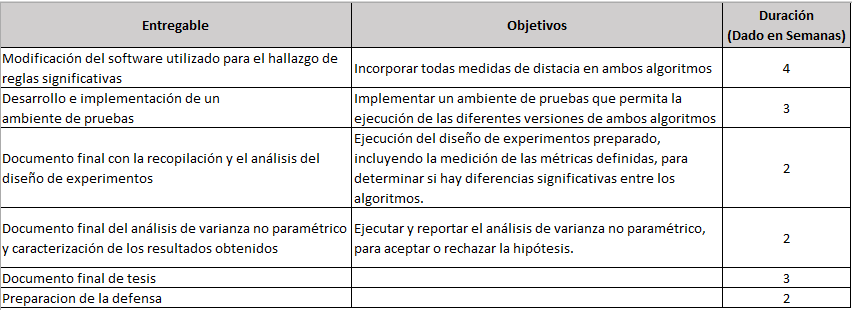
\includegraphics[scale=0.7]{deliverables.png}\\
\end{center}
\end{table}
\begin{table}[h]
\caption{Cronograma}
\label{arm:tabla}
\begin{center}
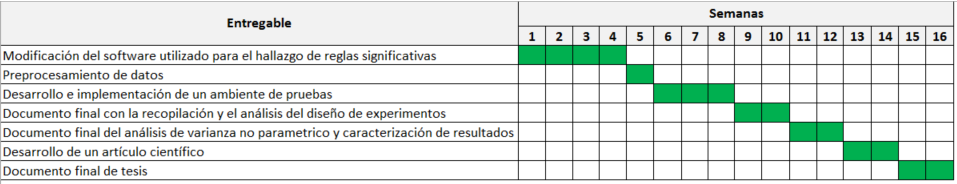
\includegraphics[scale=0.62]{projectPlan.png}\\
\end{center}
\end{table}
\clearpage
\newpage

\section{Lista de Figuras}
\begin{figure}[h]
\vspace{0.1in}
\begin{center}
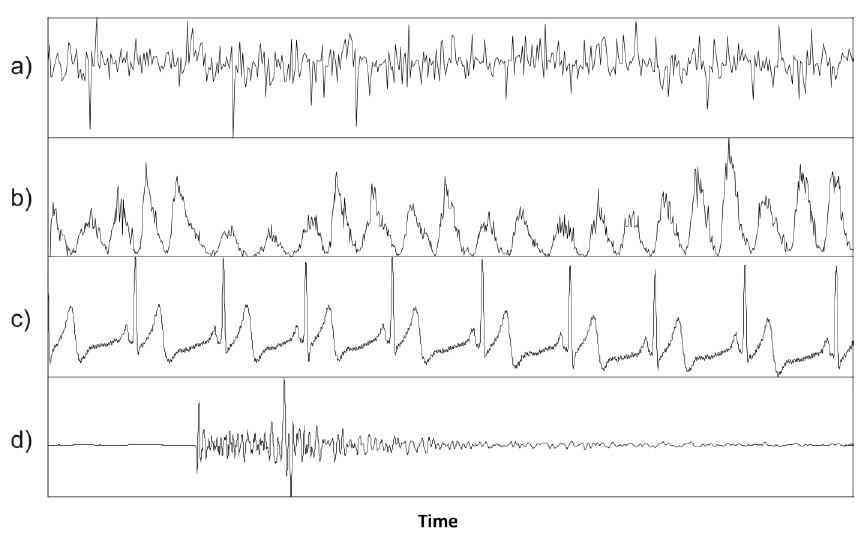
\includegraphics[scale=0.6]{timeSeries.png}\\%
\end{center}
\caption{Ejemplos de Series Temporales}
\label{arm:fig1}
\end{figure}
\begin{figure}[h]
\vspace{0.1in}
\begin{center}
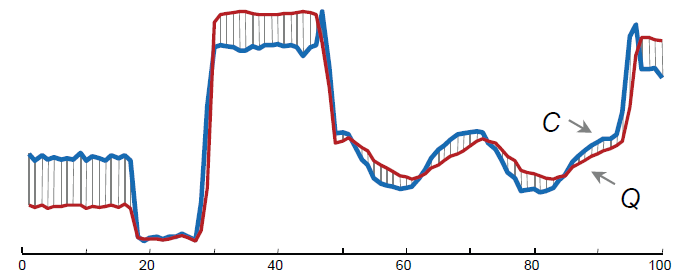
\includegraphics[scale=0.6]{euclidean.png}\\
\end{center}
\caption{Visualizaci\'on de la distancia Euclidiana de dos series temporales.}
\label{arm:fig2}
\end{figure}
\begin{figure}[h]
\vspace{0.1in}
\begin{center}
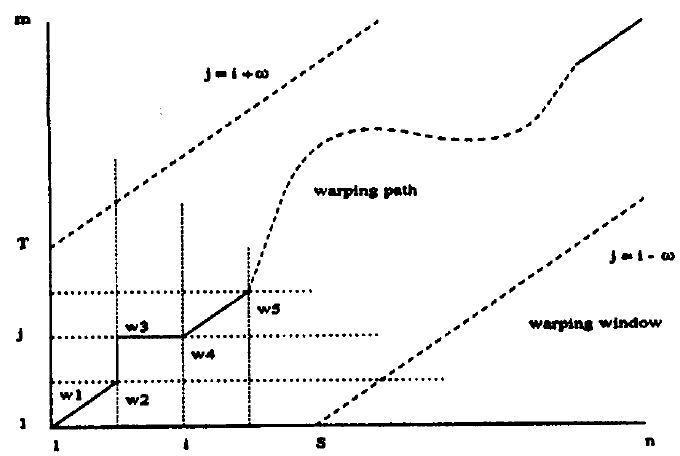
\includegraphics[scale=0.6]{dtw.png}\\
\end{center}
\caption{Visualizaci\'on de la minimizaci\'on de una ruta en DTW.}
\label{arm:fig3}
\end{figure}
\begin{figure}[h]
\vspace{0.1in}
\begin{center}
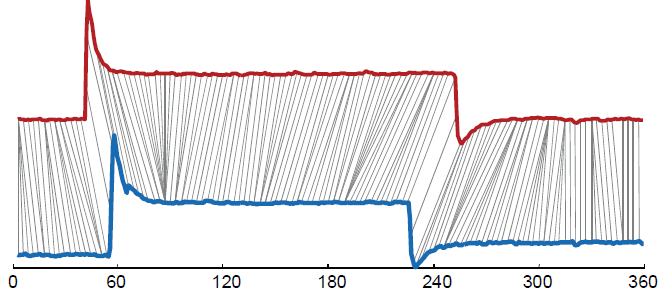
\includegraphics[scale=0.6]{dtw2.png}\\
\end{center}
\caption{Visualizaci\'on del calculo de DTW.}
\label{arm:fig4}
\end{figure}
\begin{figure}[h]
\vspace{0.1in}
\begin{center}
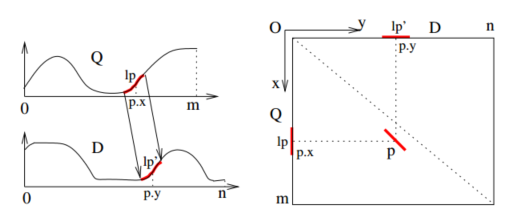
\includegraphics[scale=0.6]{spade.png}\\
\end{center}
\caption{Ejemplo del c\'alculo de LPM.}
\label{arm:fig5}
\end{figure}
\begin{figure}[h]
\vspace{0.1in}
\begin{center}
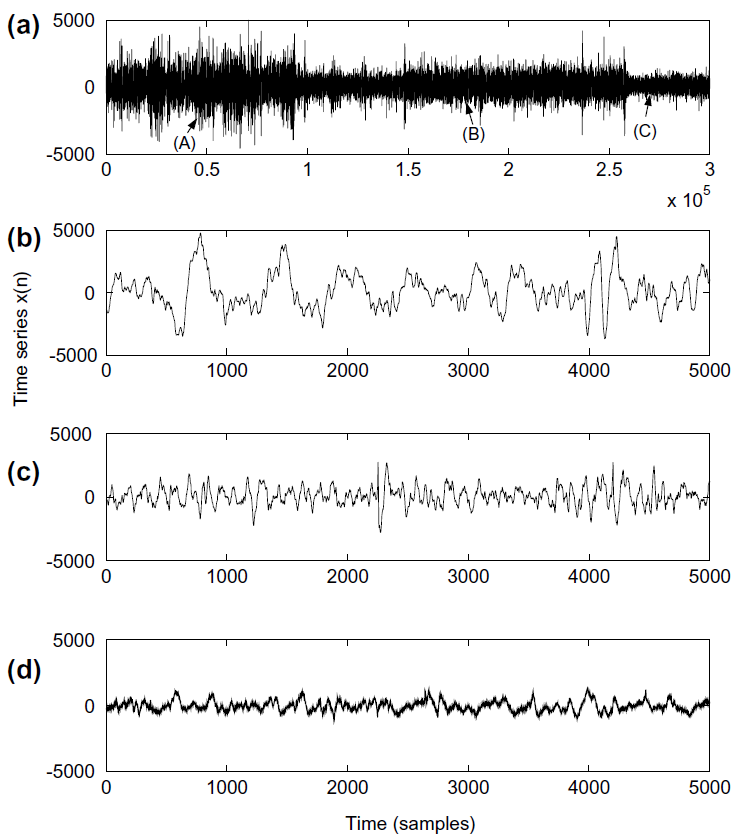
\includegraphics[scale=0.6]{brainsignal.png}\\
\end{center}
\caption{Ejemplo de ruido en las se\~nales de un electoencefalograma.}
\label{arm:fig6}
\end{figure}
\begin{thebibliography}{9}
\bibitem{rulediscovery} 
Shokoohi-Yekta, Chen, Bilson, Bing Hu, Zakaria and Eamonn Keogh. University of California, Riverside. \textit{"Discovery of Meaningful Rules in Time Series".} KDD 2015, Proceedings of the 21th ACM SIGKDD. International Conference on Knowledge Discovery and Data Mining. Pages 1085-1094.
\bibitem{montgomeryx} 
D. C. Montgomeryx.
\textit{"Guidelines for designing experiments, design and analysis of experiments."} 5th Edition, 2000, pp. 13-17".
\bibitem{statisticaldesignofexperiments} 
R. L. Mason. \textit{"Statistical Design and Analysis of Experiments With Applications to Engineering and Science."} Second Edition. John Wiley \& Sons. 2003.
\bibitem{multidimensional} 
M. Vlachos, G. Kollios, and D. Gunopulos. \textit{"Discovering similar multidimensional trajectories."} Proc 18th Int. Conf. Data Eng. pp. 673–684, 2002.
\bibitem{timewarping} 
S. Chu, E. Keogh, and D. Hart, \textit{"Iterative Deepening Dynamic Time Warping for Time Series"}. pp. 195–212, 2002.
\bibitem{DTWcubicsplineinterpolation} 
H. Li, X. Wan, Y. Liang, and S. Gao. \textit{"Dynamic Time Warping Based on Cubic Spline Interpolation for Time Series Data Mining."} 2014 IEEE Int. Conf. Data Min. Work., pp. 19–26, 2014.
\bibitem{timewarping}
C. Ratanamahatana and E. Keogh, \textit{"Everything you know about dynamic time warping is wrong."} Third Work. Min. Temporal Seq. Data, pp. 22–25, 2004.
\bibitem{indexing} 
G. Al-Naymat, S. Chawla, and J. Taheri. \textit{"SparseDTW: A novel approach to speed up dynamic time warping."} Conf. Res. Pract. Inf. Technol. Ser., vol. 101, no. December 2003, pp. 117–127, 2009.
\bibitem{distances} 
H. Ding, G. Trajcevski, and P. Scheuermann, \textit{"Querying and mining of time series data: experimental comparison of representations and distance measures."} Proc. VLDB Endow., vol. 1, no. 2, pp. 1542–1552, 2008.
\bibitem{distances} 
A. Mueen, E. Keogh, Q. Zhu, S. Cash, and B. Westover, \textit{"Exact Discovery of Time Series Motifs"}. Proc. 2009 SIAM Int. Conf. Data Min., pp. 473–484, 2009.
\bibitem{patterns} 
A. M. Denton, C. A. Besemann, and D. H. Dorr, \textit{"Pattern-based time-series subsequence clustering using radial distribution functions."} Knowl. Inf. Syst. Vol. 18, no. 1, pp. 1–27, 2009.
\bibitem{noise}
J. Hu, J. B. Gao, and K. D. White, \textit{"Estimating measurement noise in a time series by exploiting nonstationarity."} vol. 22, pp. 807–819, 2004.
\bibitem{rulediscovery}
G. Das, K. Lin, H. Mannila, G. Renganathan, and P. Smyth. \textit{"Rule discovery from time series."} Knowl. Discov. Data Min, pp. 16–22, 1998.
\bibitem{timewarping}
G. Al-Naymat, S. Chawla, and J. Taheri. \textit{"SparseDTW: A novel approach to speed up dynamic time warping."} Conf. Res. Pract. Inf. Technol. Ser., vol. 101, no. December 2003, pp. 117–127, 2009.
\bibitem{timewarpingindexing}
E. Keogh, Exact indexing of dynamic time warping, in: Processings
of the 28th VLDB Conference, 2005, pp.358-380.
\end{thebibliography}
\addcontentsline{toc}{section}{Bibliography}
%------------------------------------------------------------------------
\end{document}
%------------------------------------------------------------------------